% ==================================================================
% Chapter 1 — Introduction  (writer W1)
% ==================================================================
\chapter{Introduction}\label{ch:intro}

% ------------------------------------------------------------------
\section{Chapter overview}\label{sec:intro-overview}

This chapter describes urban congestion in Sri Lanka and the limitations of fixed-time signals, then narrows to the Maviththara junction on the Piliyandala bypass, where the specific problem and research gap are stated. The research question, motivation, aim and objectives follow, and a rich picture summarises the proposed solution, \prism{} (Pressure-based Real-time Intersection Signal Management). The chapter closes with the resources used, the project scope and an outline of the remaining chapters.

% ------------------------------------------------------------------
\section{Problem background}\label{sec:intro-background}

Road congestion is one of the most persistent constraints on economic and social life in the Colombo Metropolitan Region (CMR). The Urban Transport System Development Project for the Colombo Metropolitan Region and Suburbs, conducted by the Japan International Cooperation Agency together with the Ministry of Transport, documented a rapidly growing private fleet, a declining public-transport share and severe peak-period congestion on the corridors feeding the city, and projected further deterioration without investment in infrastructure and traffic management~\cite{jica2014comtrans}. More recent studies confirm the trend: CMR commuters report losses of time, fuel, earnings and productivity~\cite{dammulla2022colombo}, and the cost of lost workforce time and excess fuel is a substantial drain on the regional economy~\cite{jayasooriya2017congestion}. Kumarage~\cite{kumarage2022policy} further argues that Sri Lankan transport policy has for decades lacked effective, evidence-based direction, so that operational improvements have lagged behind demand.

The composition of the Sri Lankan fleet makes the problem distinctive. Of more than \est{9.2~million} registered vehicles, over \est{5.2~million} are motorcycles~\cite{newsfirst2026motorcycles}, and motorcycles accounted for \est{223,228} of the \est{312,177} new registrations in 2025 alone, when vehicle imports resumed after the economic crisis~\cite{dailymirror2026registrations,dmt_stats}. Three-wheelers form a further large, distinctively South Asian class. These small vehicles share the carriageway with cars, buses and lorries without strict lane discipline, filtering between larger vehicles to the stop line. A queue of twenty motorcycles and one of twenty buses differ greatly in length and discharge time, which is why traffic engineers express demand in Passenger Car Units (PCU) that weight each class by its effect on capacity~\cite{irc106,hcm2016}. Recent Sri Lankan measurements confirm that locally derived equivalence factors differ markedly from foreign defaults~\cite{perera2025pce}.

Most signalised junctions in the CMR are operated by \emph{fixed-time} controllers, which repeat a predetermined cycle with constant green intervals regardless of the traffic actually present. Fixed plans are classically derived from Webster's delay formula~\cite{webster1958} using historical counts and perform reasonably only when demand is stable~\cite{papageorgiou2003review}. Suburban Colombo demand is not stable: school traffic, office shifts, bus bunching and incidents produce surges a fixed plan cannot detect, so one approach queues for hundreds of metres while another, almost empty, receives green. When the plan visibly fails, traffic police officers switch the signals off and direct traffic by hand. Manual control works because the officer responds to visible queues, but it is labour-intensive, inconsistent and hazardous, and its prevalence shows that responsiveness to queues is exactly what the installed controllers lack. Adaptive Traffic Signal Control (ATSC) systems such as SCOOT~\cite{hunt1981scoot} and SCATS~\cite{sims1980scats} have provided this responsiveness elsewhere for decades, but they depend on dense inductive-loop detection, proprietary hardware and lane-disciplined traffic, and they have seen little adoption in Sri Lanka.

% ------------------------------------------------------------------
\section{Problem statement}\label{sec:intro-problem}

\subsection{General problem}\label{sec:intro-general}

Signalised junctions in Sri Lankan cities allocate green time without measuring demand, and the commercial adaptive systems that could respond were designed for lane-disciplined traffic and loop detectors that cannot see filtering motorcycles. Recent local work has begun to apply artificial intelligence and Reinforcement Learning (RL) to signal timing in Sri Lanka~\cite{wijesekara2025signals,shangeeth2025emission}, but RL controllers require large amounts of training interaction, behave as black boxes and offer no guaranteed bounds on safety or fairness, which remains a major obstacle to their deployment by road authorities~\cite{noaeen2022rl}. Road users therefore face long, unpredictable waits, and police officers substitute for the controller at the busiest times.

\subsection{Specific problem}\label{sec:intro-specific}

This research concentrates on the Maviththara junction in Piliyandala, Colombo District, where the Piliyandala bypass (the main road) crosses a local cross road (\cref{fig:intro-site}). Every arm has two inbound and two outbound lanes, and because Sri Lanka drives on the left, right-turning vehicles must cross the opposing stream. Each corner has a channelised left-turn slip lane controlled by give-way rather than by the signals. Opposite approaches of the same road are served together, giving four signal phases: $\phi_1$ bypass through, $\phi_2$ bypass protected right turn, $\phi_3$ cross-road through and $\phi_4$ cross-road protected right turn.

\begin{figure}[htbp]
  \centering
  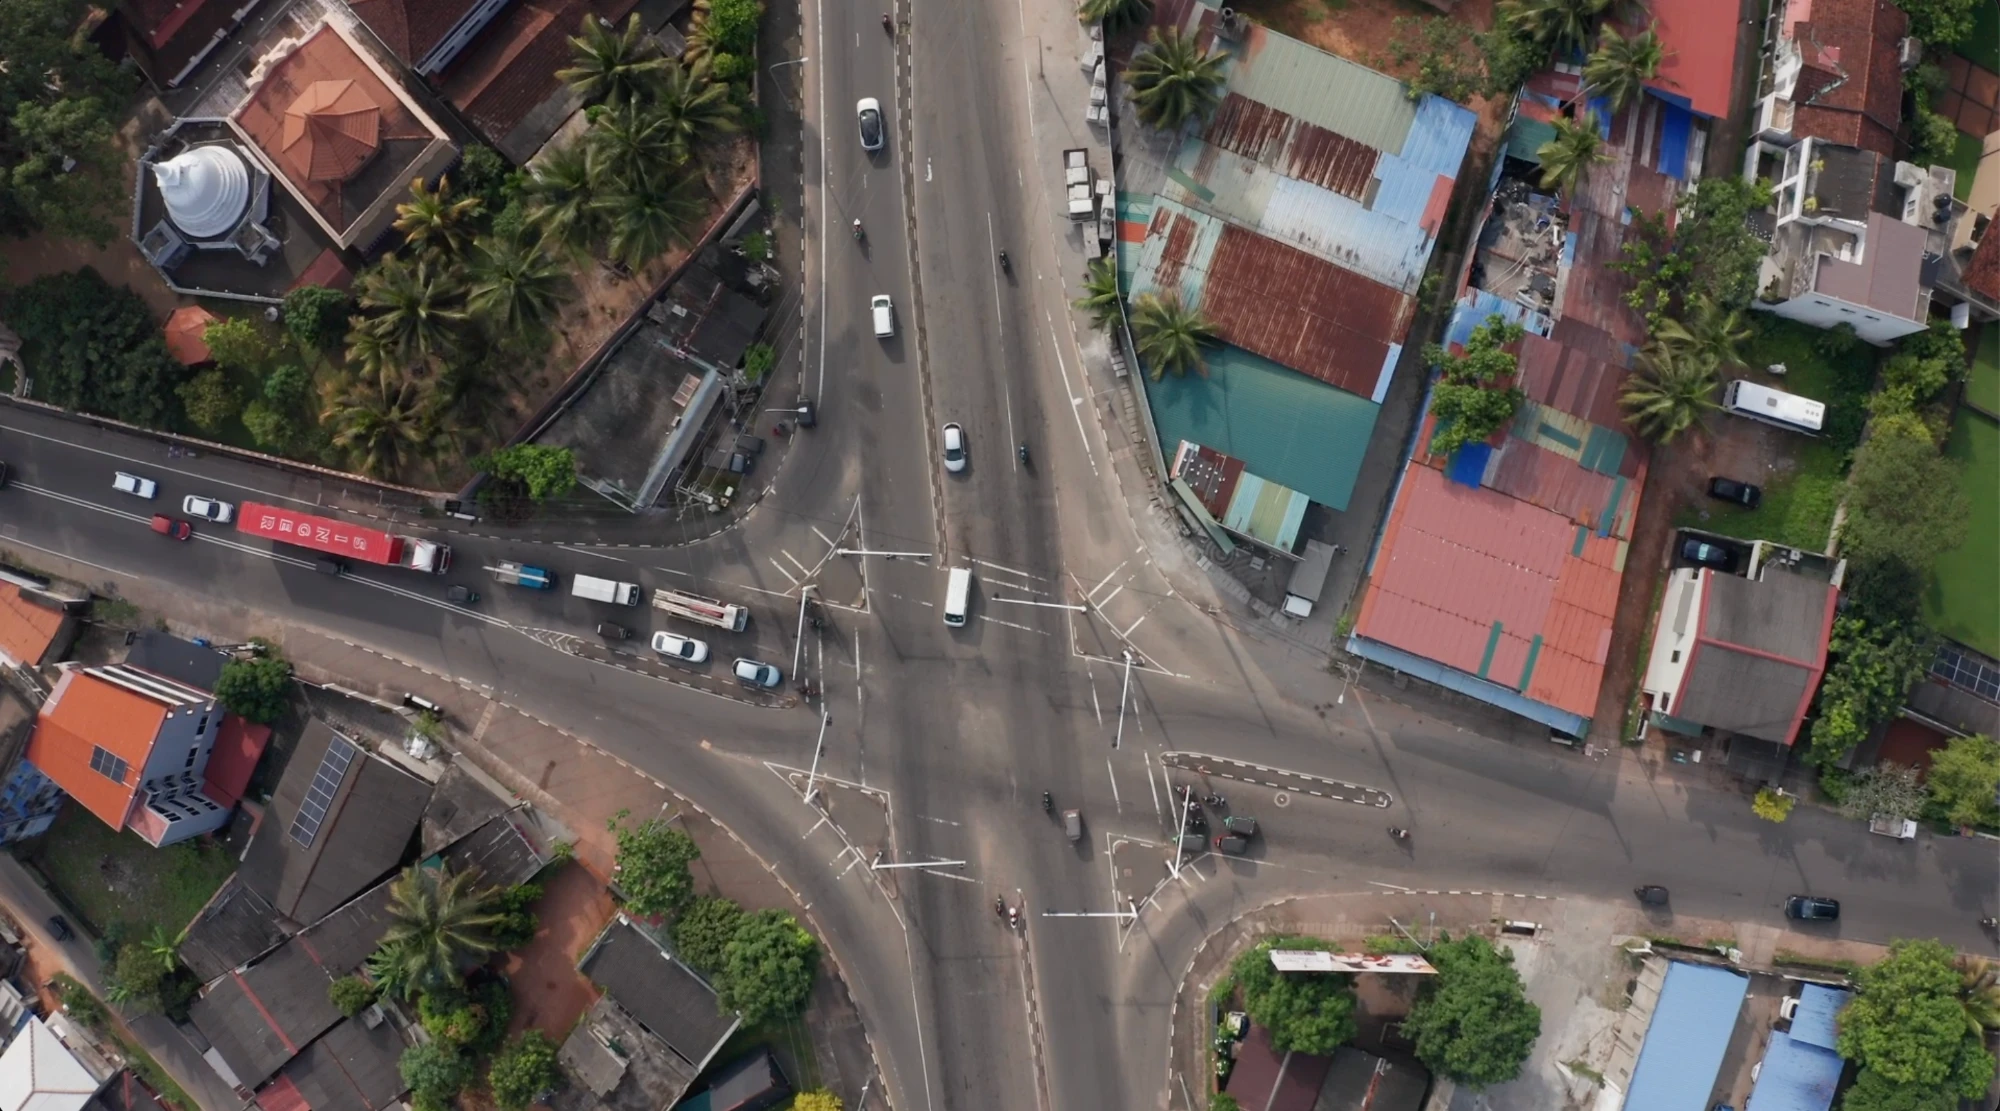
\includegraphics[width=\textwidth]{figures/junction_clean.png}
  \caption{Aerial view of the Maviththara junction, Piliyandala, taken as a nadir (straight-down) image from the DJI Mini 2 drone during the survey of 2 October 2026; the Piliyandala bypass and the cross road meet diagonally, with channelised left-turn slip lanes at each corner}
  \label{fig:intro-site}
\end{figure}

Observation of the junction established the existing fixed-time plan. Each phase is followed by an intergreen of 3~s amber and an all-red interval, assumed in this research to be 2~s because it could not be timed reliably from the footage. The bypass through phase $\phi_1$ receives 21~s of green (red 54~s) and the bypass right-turn phase $\phi_2$ 8~s (red 67~s), giving a cycle of $21 + 3 + 54 = 78$~s. The cross-road through green follows from its observed red of 60~s as $78 - 3 - 60 = 15$~s. The green of $\phi_4$ could not be timed directly and was derived from the cycle constraint $21 + 8 + 15 + G_4 + 4 \times 5 = 78$, which gives $G_4 = $ \est{14~s}. The same cycle runs in the saturated morning peak and in the moderate afternoon. Waiting times measured from the drone footage under this plan averaged \est{104.7~s} per vehicle in the morning peak and \est{46.3~s} in the early afternoon, with observed demand of \est{3,420~veh/h} and \est{2,280~veh/h} respectively, motorcycles and three-wheelers together forming \est{62\%} of the morning flow.

At the heaviest periods the Piliyandala Traffic Police switch the lights off and direct traffic manually. In a discussion held on 17 September 2026, the Piliyandala Traffic Police and the Road Development Authority (RDA) expressed two needs: (a) to reduce the time that traffic police officers spend managing the junction manually, and (b) to reduce the waiting time of every road user. Emergency vehicles currently rely on other traffic making way, and no priority logic was requested at this stage.

Making the junction adaptive requires both \emph{sensing} and a \emph{control law}. Inductive loops measure presence at a point, cannot reliably detect filtering motorcycles and require cutting the road surface; cameras suffer under glare, rain and darkness and capture faces and number plates. A pole-mounted Light Detection and Ranging (LiDAR) sensor measures the position of every object directly~\cite{zhao2019lidar,lv2019lidar}, but it is expensive, and procuring one before demonstrating its benefit at this site would be irresponsible. The \textbf{research gap} is therefore as follows: no existing work has designed and evaluated a transparent, mathematically defined adaptive controller that (i) weights heterogeneous Sri Lankan traffic by PCU, (ii) operates on realistic, imperfect LiDAR observations, (iii) guarantees safety and bounded fairness, and (iv) is evaluated on a simulation model of a real Sri Lankan junction calibrated against per-vehicle waiting times measured from drone video. This research addresses that gap at the Maviththara junction.

% ------------------------------------------------------------------
\section{Research question}\label{sec:intro-rq}

The research was guided by one principal question and three sub-questions.

\textbf{Research question (RQ):} \emph{How can a LiDAR-driven, PCU-weighted, pressure-based adaptive signal controller, calibrated with drone-observed heterogeneous traffic, reduce the average waiting time of road users at the Maviththara junction compared with the existing fixed-time signal plan?}

{\emergencystretch=2em\begin{description}[leftmargin=1.7cm, labelwidth=1.3cm, labelsep=0.4cm, itemsep=2pt]
  \item[SRQ1] What are the demand, composition, turning and waiting characteristics of traffic at the Maviththara junction, and how can they be extracted reliably from nadir drone video?
  \item[SRQ2] How can a purely mathematical control law account for heterogeneous vehicle classes, fairness between phases and imperfect LiDAR sensing?
  \item[SRQ3] How does the proposed controller perform against fixed-time, actuated and Webster-optimised control, and how sensitive is it to sensor noise and to its own parameters?
\end{description}}

% ------------------------------------------------------------------
\section{Research motivation}\label{sec:intro-motivation}

The motivation is both personal and societal. A commuter leaving Piliyandala for Colombo at 07:00 spends much of the journey stationary at isolated fixed-time junctions, Maviththara among the first, and every unnecessary second of red is multiplied by thousands of vehicles per peak hour. The author's long-term vision is that every major junction should be equipped with a LiDAR sensor and an adaptive controller, so that neighbouring junctions can share predicted platoons and a commuter who leaves home can reach the destination in the minimum possible time. Decentralised max-pressure control~\cite{varaiya2013maxpressure}, on which \prism{} builds, suits this vision because it needs only local information yet carries network-level throughput guarantees. This thesis is the first, single-junction step towards that goal.

LiDAR was chosen as the target sensor for three reasons. First, it records geometry rather than appearance, capturing the shape, position and speed of a vehicle but not faces or number plates, so a controller that depends only on LiDAR data is privacy-preserving by construction. Second, it is an active sensor that works equally at night and under strong tropical sunlight. Third, it measures position and distance to the stop line directly, rather than inferring them from image coordinates, which allows queues to be measured in PCU over the whole approach.

Finally, machine learning was deliberately kept out of the control loop and used only offline to detect vehicles in drone video. The signal decision is computed by explicit equations whose every output can be explained to a traffic engineer, whose safety and fairness can be bounded and certified, and which require no training data, an important advantage in a country where no historical detector data exist for most junctions~\cite{noaeen2022rl}.

% ------------------------------------------------------------------
\section{Research aim}\label{sec:intro-aim}

To design, implement and evaluate a LiDAR-driven, PCU-weighted, pressure-based adaptive traffic signal controller (\prism{}) that reduces the waiting time of all road users at the Maviththara junction, using a SUMO model calibrated with drone-observed Sri Lankan traffic.

% ------------------------------------------------------------------
\section{Research objectives}\label{sec:intro-objectives}

The aim was decomposed into seven objectives, listed in \cref{tab:intro-objectives}. Their accomplishment is assessed in \cref{ch:conc}.

\begin{table}[htbp]
  \centering
  \caption{Research objectives}
  \label{tab:intro-objectives}
  \small
  \renewcommand{\arraystretch}{1.15}
  \begin{tabularx}{\textwidth}{@{}l X l@{}}
    \toprule
    \textbf{ID} & \textbf{Objective} & \textbf{SRQ} \\
    \midrule
    O1 & To identify the operational problems of the Maviththara junction and the needs of its stakeholders through literature, observation and discussion with the Piliyandala Traffic Police and the RDA. & SRQ1 \\
    O2 & To analyse existing adaptive signal control systems, control algorithms, sensing technologies and simulation tools critically, and to identify the research gap. & SRQ2 \\
    O3 & To design and develop a drone-video trajectory extraction pipeline (DTX) that measures demand, composition, turning ratios, saturation flow and per-vehicle waiting time. & SRQ1 \\
    O4 & To develop a SUMO model of the junction, first verified with mock demand and then calibrated and validated with the drone-extracted data. & SRQ1 \\
    O5 & To design and implement a Virtual LiDAR Sensor (VLS) that reproduces realistic LiDAR noise, dropout, occlusion and size-class confusion. & SRQ2 \\
    O6 & To design and implement the PRISM control algorithm with guaranteed safety, bounded fairness and explainable decisions, using mathematics only (no machine learning in control). & SRQ2 \\
    O7 & To evaluate PRISM against fixed-time (B1), actuated (B2) and Webster-optimised (B3) control and an oracle-sensor variant (PRISM-GT), with statistical testing and sensitivity analysis. & SRQ3 \\
    \bottomrule
  \end{tabularx}
\end{table}

% ------------------------------------------------------------------
\section{Rich picture of the proposed solution}\label{sec:intro-richpicture}

\Cref{fig:intro-richpicture} presents a rich picture of the proposed solution, emphasising its workflow and the stakeholders around it.

\begin{figure}[htbp]
  \centering
  \resizebox{\textwidth}{!}{%
  \begin{tikzpicture}[
      font=\linespread{1.0}\selectfont\sffamily\small,
      box/.style={font=\linespread{1.0}\selectfont\sffamily\small, draw, rounded corners=3pt, fill=black!5, align=center, text width=3.3cm, minimum height=1.55cm, inner sep=3pt},
      hl/.style={box, very thick, fill=black!12},
      sh/.style={draw, ellipse, dashed, align=center, inner sep=2pt, font=\sffamily\footnotesize, fill=white},
      flow/.style={-{Stealth[length=2.6mm]}, thick},
      soft/.style={-{Stealth[length=2.2mm]}, dashed, black!65},
      lab/.style={font=\sffamily\scriptsize, align=center, fill=white, inner sep=1pt}
    ]
    % ---- workflow row 1
    \node[box] (drone) at (0,0) {\textbf{1. Drone survey}\\[1pt]\scriptsize DJI Mini 2, 4K@30\,fps,\\ \scriptsize nadir view, 02.10.2026\\ \scriptsize morning \& afternoon};
    \node[box] (dtx) at (4.6,0) {\textbf{2. \dtx{}}\\[1pt]\scriptsize stabilise, YOLOv8+SAHI,\\ \scriptsize ByteTrack, homography,\\ \scriptsize waiting times};
    \node[box] (sumo) at (9.2,0) {\textbf{3. Calibrated \sumo{} model}\\[1pt]\scriptsize 2+2 lanes, slip lanes,\\ \scriptsize sublane, 7 classes, GEH};
    \node[box] (vls) at (13.8,0) {\textbf{4. \vls{}}\\[1pt]\scriptsize virtual LiDAR on 6\,m pole,\\ \scriptsize $R=75$\,m, noise, dropout,\\ \scriptsize occlusion};
    % ---- workflow row 2
    \node[hl] (prism) at (13.8,-3.3) {\textbf{5. \prism{} controller}\\[1pt]\scriptsize PCU pressure, urgency,\\ \scriptsize $G_{\min}$/$G_{\max}$, fail-safe};
    \node[box] (heads) at (9.2,-3.3) {\textbf{6. Signal heads}\\[1pt]\scriptsize $\phi_1$--$\phi_4$, 3\,s amber\\ \scriptsize + 2\,s all-red};
    \node[box] (eval) at (4.6,-3.3) {\textbf{7. Evaluation}\\[1pt]\scriptsize 10 seeds, waiting time,\\ \scriptsize queues, Wilcoxon test};
    \node[box] (base) at (0,-3.3) {\textbf{Baselines}\\[1pt]\scriptsize B1 fixed 78\,s, B2 actuated,\\ \scriptsize B3 Webster, PRISM-GT};
    % ---- mock data (development order)
    \node[box, dashed, fill=white, text width=3.0cm, minimum height=1.1cm] (mock) at (9.2,2.45) {\textbf{Mock demand}\\ \scriptsize 300/500/700 veh/h, even split};
    % ---- arrows
    \draw[flow] (drone) -- node[lab, above=2pt]{video} (dtx);
    \draw[flow] (dtx) -- node[lab, above=2pt]{routes,\\ KPIs} (sumo);
    \draw[soft] (mock) -- node[lab, right=1pt]{stage 1\\ (first)} (sumo);
    \draw[flow] (sumo) -- node[lab, above=2pt]{vehicle\\ states} (vls);
    \draw[flow] (vls) -- node[lab, right=2pt]{object list\\ every 1\,s} (prism);
    \draw[flow] (prism) -- node[lab, above=2pt]{phase\\ decision} (heads);
    \draw[flow] (heads) -- node[lab, right=2pt]{TraCI} (sumo);
    \draw[flow] (sumo.south west) ++(0.3,0) -- node[lab, left=2pt, pos=0.45]{KPIs} (eval.north east);
    \draw[flow] (base) -- (eval);
    \node[lab, font=\sffamily\scriptsize\itshape] at (6.9,-0.55) {stage 2\\ (last)};
    % ---- stakeholders
    \node[sh] (reg) at (0,2.45) {CAASL / MoD\\ (regulators)};
    \node[sh] (police) at (4.6,2.45) {Piliyandala\\ Traffic Police};
    \node[sh] (rda) at (13.8,2.45) {Road Development\\ Authority (RDA)};
    \node[sh] (comm) at (9.2,-5.7) {Commuters: motorcyclists,\\ three-wheelers, cars, buses};
    \draw[soft] (reg) -- node[lab, right=1pt]{flight approval} (drone);
    \draw[soft] (police.south west) -- node[lab, above left=0pt and 0pt, pos=0.35]{permission} (drone.north east);
    \draw[soft] (police) -- node[lab, right=1pt]{needs (17.09.2026)} (dtx);
    \draw[soft] (rda) -- node[lab, right=1pt]{needs (17.09.2026)} (vls);
    \draw[soft] (eval.south) |- node[lab, pos=0.3, left=2pt]{less waiting,\\ fewer manual-\\control periods} (comm.west);
    \draw[soft] (heads) -- node[lab, right=2pt]{green time} (comm);
  \end{tikzpicture}}
  \caption{Rich picture of the proposed solution: drone survey, \dtx{} extraction, calibrated \sumo{} model, virtual LiDAR (\vls{}), the \prism{} controller acting on the signal heads in a closed loop, and evaluation against the baselines, with the stakeholders around the workflow}
  \label{fig:intro-richpicture}
\end{figure}

The workflow begins with a drone survey of the junction, approved by the Civil Aviation Authority of Sri Lanka (CAASL) and the Ministry of Defence (MoD) and supported by the Piliyandala Traffic Police. The Drone Trajectory eXtractor (\dtx{}) converts the nadir video into georeferenced vehicle trajectories, from which demand, composition, turning ratios, saturation flow and per-vehicle waiting times are derived. These quantities calibrate a microscopic model of the junction in Simulation of Urban MObility (\sumo{})~\cite{lopez2018sumo}. Inside the simulation, a Virtual LiDAR Sensor (\vls{}) mounted on a pole at the junction centre produces a noisy object list every second, and the \prism{} controller, which sees only that list and never the simulator's ground truth, selects phases that are applied to the signal heads through the Traffic Control Interface (TraCI). The resulting indicators are compared with the three baselines and an oracle-sensor variant. Around the workflow, the police and the RDA supplied the needs, the regulators authorised the flights, and commuters benefit from reduced waiting.

The development order is also shown. Because the drone flights could only take place late in the project, all components were first developed and verified with \emph{mock data}, in which traffic was split evenly across the four approaches at 300, 500 and 700~veh/h. This allowed the network, sensor and controller to be built, safety-tested and tuned before real data existed. The drone data came last, replacing the mock demand and calibrating the model before the definitive experiments.

% ------------------------------------------------------------------
\section{Resource requirements}\label{sec:intro-resources}

\subsection{Hardware requirements}\label{sec:intro-hardware}

The hardware used is listed in \cref{tab:intro-hardware}. Detector training used a cloud Graphics Processing Unit (GPU); all other work ran on a student laptop. A physical LiDAR sensor was specified as the eventual deployment target but was not purchased.

\begin{table}[htbp]
  \centering
  \caption{Hardware requirements}
  \label{tab:intro-hardware}
  \small
  \renewcommand{\arraystretch}{1.15}
  \begin{tabularx}{\textwidth}{@{}p{3.4cm} p{4.6cm} X@{}}
    \toprule
    \textbf{Item} & \textbf{Specification} & \textbf{Purpose} \\
    \midrule
    Student laptop & \est{Intel Core i7 (8 cores)}, \est{16~GB memory}, \est{512~GB SSD} & Development, \dtx{} inference, \sumo{} simulation and batch experiments \\
    Google Colab GPU & NVIDIA T4, 16~GB & Fine-tuning YOLOv8 on annotated drone frames \\
    DJI Mini 2 drone & 4K video at 30~fps, hovering nadir view & Recording the morning and afternoon survey sessions (flown by a CAASL-registered operator) \\
    Roadside LiDAR (future) & 32-channel 360\textdegree{} unit, e.g.\ Ouster OS1-32~\cite{ouster_os1} & Target sensor for a real deployment; not purchased, emulated by \vls{} \\
    \bottomrule
  \end{tabularx}
\end{table}

\subsection{Software requirements}\label{sec:intro-software}

The software stack, listed in \cref{tab:intro-software}, consists entirely of free and open-source or free-tier tools, which keeps the solution reproducible and affordable for a public authority.

\begin{table}[htbp]
  \centering
  \caption{Software requirements}
  \label{tab:intro-software}
  \small
  \renewcommand{\arraystretch}{1.15}
  \begin{tabularx}{\textwidth}{@{}p{4.4cm} X@{}}
    \toprule
    \textbf{Software} & \textbf{Purpose} \\
    \midrule
    Python 3.11 & Main implementation language for \dtx{}, \vls{}, \prism{} and the experiment harness \\
    Ultralytics YOLOv8~\cite{jocher2023yolov8} & Vehicle detection in drone frames (seven classes) \\
    SAHI~\cite{akyon2022sahi} & Sliced (tiled) inference for small objects such as motorcycles \\
    supervision (ByteTrack)~\cite{zhang2022bytetrack} & Multi-object tracking with persistent vehicle identities \\
    OpenCV & Video input/output, feature matching, stabilisation and homography \\
    NumPy, SciPy, Pandas & Numerical computation, smoothing, statistics and tabular data \\
    Matplotlib & Plots of results and diagnostics \\
    \sumo{} \est{1.20.0} with TraCI / libsumo~\cite{lopez2018sumo,wegener2008traci} & Microscopic traffic simulation and online signal control \\
    netedit & Editing the junction network, lanes, slip lanes and signal program \\
    pytest & Automated unit and integration tests \\
    Git and GitHub & Version control and backup of code and configuration \\
    CVAT / Roboflow & Annotation of drone frames for detector fine-tuning \\
    Google Colab & Cloud notebook environment for GPU training \\
    \LaTeX{} & Typesetting of this thesis \\
    \bottomrule
  \end{tabularx}
\end{table}

% ------------------------------------------------------------------
\section{Project scope}\label{sec:intro-scope}

The scope was bounded to suit an undergraduate timeframe; \cref{tab:intro-scope} summarises what was and was not included.

\begin{table}[htbp]
  \centering
  \caption{Project scope}
  \label{tab:intro-scope}
  \small
  \renewcommand{\arraystretch}{1.15}
  \begin{tabularx}{\textwidth}{@{}X X@{}}
    \toprule
    \textbf{In scope} & \textbf{Out of scope} \\
    \midrule
    One junction (Maviththara, Piliyandala bypass) & Coordination of a network of junctions \\
    Simulated LiDAR (\vls{}) with a realistic error model & Purchase and deployment of real LiDAR hardware \\
    Two drone sessions (morning peak, afternoon) & The approved evening session (lost to bad weather) \\
    Four-phase control ($\phi_1$--$\phi_4$) with fixed intergreens & Emergency-vehicle pre-emption \\
    Left-turn slip lanes modelled as unsignalised give-way links & Pedestrian phases and pedestrian modelling \\
    Mock-data development followed by drone calibration & Simulation of police manual control \\
    Results visualised in \sumo{}-GUI & A custom web dashboard \\
    Pure-mathematics control (\prism{}) & Machine-learning or RL-based control \\
    \bottomrule
  \end{tabularx}
\end{table}

Only the Maviththara junction was modelled; spillback from neighbouring junctions was represented only through the boundary conditions observed in the footage. No physical sensor was installed and no live signal was controlled: all control took place in \sumo{}, with the LiDAR represented by \vls{}, so that the benefit could be quantified before any money is spent on hardware. Real data came from two sessions flown on 2 October 2026, the morning peak (07:00--08:00) and the afternoon (13:30--14:30). The evening session (17:00--18:00) was approved but could not be recorded because of bad weather, so evening, weekend and wet-weather conditions remain unobserved. The existing four-phase structure was retained for all controllers so that differences in performance can be attributed to timing decisions rather than to changes in phasing or geometry, and the slip lanes were left unsignalised as they are on site. Pedestrians were not modelled; a pedestrian minimum-green parameter exists in the controller but was not exercised. Manual police control was used as motivation but not simulated, because an officer's decisions cannot be reproduced reliably. Emergency-vehicle pre-emption, network coordination and a web dashboard are deferred to future work, and results are presented through the \sumo{} graphical interface only. Machine learning was confined to vehicle detection.

% ------------------------------------------------------------------
\section{Chapter summary}\label{sec:intro-summary}

This chapter described congestion and fixed-time control in Sri Lanka, defined the specific problem at the Maviththara junction and the research gap, and presented the research question, motivation, aim, objectives, rich picture, resources and scope. The remainder of the thesis is organised as follows. \Cref{ch:lit} critically reviews existing signal control systems, control algorithms, sensing technologies and simulation tools, and justifies the research gap. \Cref{ch:method} explains the research paradigm, the Design Science Research strategy, the data collection mechanisms, project management and ethical considerations. \Cref{ch:srs} analyses the stakeholders and specifies the requirements and system models. \Cref{ch:impl} presents the design and implementation of \dtx{}, the \sumo{} model, \vls{} and \prism{}. \Cref{ch:eval} reports the testing strategy and the evaluation of \prism{} against the baselines. Finally, \cref{ch:conc} assesses the accomplishment of the objectives, reflects on the work and recommends future directions.
